\section{Commissioning-Calibrated GP-HOCBF Safety-Filter Architecture}
\label{sec:method}

\subsection{Safety-Filter Workflow and Implementation Settings}

Online operation has three steps: evaluate the GP residual model, build HOCBF rows with the correct relative degrees, and solve one QP to project the proposed deviation command. Offline commissioning supplies the residual data, GP coverage checks, and scalar margin factor $\epsilon_\kappa$. The theorem states the conditions under which the full implemented-margin endpoint yields continuous-time forward invariance. Section~\ref{sec:exp} then evaluates how much of that margin should be applied under each mismatch regime.

Figure~\ref{fig:architecture} summarizes the overlay architecture. The upstream controller produces a deviation command $v_{\mathrm{prop}}$ around the LQR-stabilized equilibrium controller, and the safety filter returns the nearest admissible command $v^*$. The total actuator command is
\begin{equation}
    u_k = u_0 + K(x_0-x_k) + v_k^* ,
    \label{eq:deviation_control}
\end{equation}
where $u=[u_B,D_{fw},u_t]^\top$ denotes coal feed, feedwater flow, and turbine-valve opening. The HOCBF and QP are formulated in the deviation-input space. With $\xi=x-x_0$ and $A_K=A-BK$, the stabilized deviation model used to build the HOCBF rows is
\begin{equation}
    \dot{\xi}=A_K\xi+Bv+\Delta f_\xi(\xi).
    \label{eq:stabilized_deviation_model}
\end{equation}
Table~\ref{tab:implementation_settings} lists the measurement, constraint, GP, QP, fallback, and runtime settings used in the benchmark and plant implementation.

\begin{table}[htbp]
    \centering
    \caption{Measurement/control variables and implementation settings used by the RoCBF-SF safety filter in the fifth-order CCS benchmark and plant implementation.}
    \label{tab:implementation_settings}
    \small
    \renewcommand{\arraystretch}{0.98}
    \begin{tabular}{>{\raggedright\arraybackslash}p{0.23\textwidth}>{\raggedright\arraybackslash}p{0.24\textwidth}>{\raggedright\arraybackslash}p{0.43\textwidth}}
        \toprule
        Item & Setting & Role in the filter \\
        \midrule
        Benchmark state & State vector $x=[r_B,p_m,h_m,N_e,\tau_f]^\top$ & Five-state nominal predictor used to construct the benchmark dynamics and HOCBF rows. \\
        GP input/output & $x_k^{\mathrm{GP}}=[p_{m,k},h_{m,k},N_{e,k}]^\top$ and three residual rates & Measured constrained outputs used by both benchmark and plant GPs; all five states and three proposed controls remain inputs to the nominal one-step predictor. \\
        Manipulated inputs & Input vector $u=[u_B,D_{fw},u_t]^\top$ & Coal feed, feedwater flow, and turbine valve opening; QP optimizes the deviation command $v$. \\
        Pressure limit & Range 13--24\,MPa; relative degree $m=2$ & High-order pressure CBF with two $\psi$-levels. \\
        Enthalpy limit & Range 2670--2830\,kJ/kg; relative degree $m=1$ & Active heat-absorption safety constraint. \\
        Power tracking band & Band $N_{\mathrm{ref}}\pm50$\,MW; relative degree $m=1$ & Load-following and turbine-output safety constraint around the active dispatch target. \\
        Sampling and hold & Controller period $T_s=1$\,s; zero-order hold & Online QP solved once per controller cycle; plant-validation exports use 5\,s record spacing. \\
        GP calibration & Three 500-point Mat\'{e}rn-5/2 residual GPs with frozen input/output standardization & Learns pressure, enthalpy, and power residual-rate means and posterior uncertainties; 200 time-isolated points are retained for validation. \\
        QP implementation & qpax, row scaling, box/rate constraints, $10^{-6}$ feasibility tolerance & Projects $v_{\mathrm{prop}}$ to the nearest admissible $v^*$ and rejects non-converged or infeasible candidates. \\
        Recovery and bypass & One guarded \texttt{pressure\_low} reduced-QP retry; otherwise live DCS command & The guarded retry is outside the full-row certificate; actuator rows are never removed. \\
        Runtime deadline & Controller period and deployed task deadline both 1000\,ms & Field exports report QP and total-task timing against the deployed deadline. \\
        Plant controller platform & AMD EPYC Embedded 4565P; 64\,GB (2$\times$32\,GB) DDR5-5600 ECC; openEuler 24.03 LTS & Deployed controller compute platform; data exchange with the DCS uses Modbus TCP. \\
        Plant software stack & Python 3.11; qpax 0.1.3; SciPy 1.17.1; Kubernetes & qpax provides the online QP solve; Kubernetes manages the deployed workload. \\
        \bottomrule
    \end{tabular}
\end{table}

\paragraph{Online filtering algorithm.}
At each sampling instant, RoCBF-SF performs the following operations:
\begin{enumerate}[label=\textbf{Step \arabic*:},leftmargin=*]
    \item Read $x_k$ and the proposed deviation action $v_{\mathrm{prop},k}$.
    \item Evaluate $\mu_{\mathrm{GP}}(x_k)$ and $\sigma_{\mathrm{GP}}(x_k)$.
    \item Build mean-corrected HOCBF constraints with the correct relative degree.
    \item Propagate GP uncertainty through the $\psi$-chain to compute $\sigmatotal(x_k)$.
    \item Solve the real-time QP
    \begin{equation}
        v_k^*=\argmin_v \|v-v_{\mathrm{prop},k}\|_2^2
        \quad \mathrm{s.t.}\quad A(x_k)v \leq b(x_k)-\epsilon_\kappa\sigmatotal(x_k),\quad v\in\mathcal{V},
        \label{eq:online_qp}
    \end{equation}
    where $\mathcal{V}$ is the deviation-input box induced by actuator limits. Row scaling is applied before the numerical solve and does not change the feasible set.
    \item Apply $u_k=u_0+K(x_0-x_k)+v_k^*$ and log intervention, feasibility, and margin diagnostics.
\end{enumerate}

\paragraph{Notation summary.}
The benchmark state is $x=[r_B,p_m,h_m,N_e,\tau_f]^\top$, and $\xi=x-x_0$ is the deviation state. The physical actuator command is $u$, while $v$ is the deviation input optimized by the safety filter. The upstream controller proposes $v_{\mathrm{prop},k}$, the QP returns $v_k^*$, and Eq.~\eqref{eq:deviation_control} maps $v_k^*$ back to the physical actuator command. The HOCBF rows are written as $A(x)v\leq b(x)$ in deviation-input form. The term $\sigmatotal(x)$ is the compositional GP-HOCBF margin, and $\epsilon_\kappa$ is the commissioning factor multiplying that margin.

Both the benchmark and plant implementations use the measured-output vector
\begin{equation}
    x_k^{\mathrm{GP}}=[p_{m,k},h_{m,k},N_{e,k}]^\top .
    \label{eq:gp_input_vector}
\end{equation}
Three independent GPs model the corresponding one-step nominal-model residual rates. The benchmark target is $(x_{k+1,J_{\mathrm{GP}}}-\hat{x}^{\mathrm{nom}}_{k+1|k,J_{\mathrm{GP}}})/T_s$, where $J_{\mathrm{GP}}=\{p_m,h_m,N_e\}$. The full nominal predictor uses all five states and all three control deviations; fuel, feedwater, and turbine-valve commands are therefore represented in the nominal prediction but are not direct kernel inputs.

\paragraph{Operating-point interpretation.}
RoCBF-SF denotes the complete safety-filter design in Fig.~\ref{fig:architecture}: correct-relative-degree HOCBF rows, GP residual mean correction, compositional uncertainty propagation, QP projection, and tunable $\epsilon_\kappa$. The upstream controller may be classical or learned; the experiments evaluate the downstream filter contribution rather than the upstream controller. Experimental rows labelled GP-HOCBF and RoCBF-SF are fixed operating points or ablations. Thus, $\epsilon_\kappa=0$ tests mean correction alone, $\epsilon_\kappa=1$ tests the full implemented margin, and Section~\ref{sec:kappa} selects and evaluates the calibrated benchmark operating point.

\subsection{Mismatch Model and HOCBF Constraints}

Consider a control-affine system with model mismatch:
\begin{equation}
    \dot{x} = \underbrace{f_0(x) + g_0(x)u}_{\text{nominal}} + \underbrace{\Deltaf(x)}_{\text{residual}}, \quad x \in \R^n, \; u \in \calU \subset \R^m
    \label{eq:true}
\end{equation}
where $\Deltaf$ represents unmodeled dynamics, parameter drift, and external disturbances. The formal certificate assumes a known input matrix ($\Delta g=0$), so the GP learns drift residuals rather than uniform actuator-gain uncertainty.

The six scalar safety barriers used in the benchmark are
\begin{align}
    h_{p,L}(x)&=p_m-13,\quad h_{p,U}(x)=24-p_m, \nonumber\\
    h_{h,L}(x)&=h_m-2670,\quad h_{h,U}(x)=2830-h_m, \label{eq:barriers}\\
    h_{N,L}(x)&=N_e-(N_{\mathrm{ref}}-50),\quad h_{N,U}(x)=N_{\mathrm{ref}}+50-N_e. \nonumber
\end{align}
Pressure barriers use relative degree two, while separator-enthalpy and power barriers use relative degree one.

For a constraint $h(x) \geq 0$ with relative degree $m$, the HOCBF $\psi$-chain is:
\begin{equation}
    \psi_0 = h(x), \quad \psi_i = \dot{\psi}_{i-1} + \alpha_i(\psi_{i-1}), \;\; i=1,\ldots,m
    \label{eq:psi}
\end{equation}
With linear $\alpha_i(r)=k_i r$, substituting Eq.~\eqref{eq:deviation_control} into the stabilized model gives exact-model rows in deviation-input form, $A_0(x)v \leq b_0(x)$. This preserves the bookkeeping between pressure ($m=2$) and enthalpy/power ($m=1$) constraints while keeping the QP decision variable equal to $v$.

\begin{figure}[htbp]
    \centering
    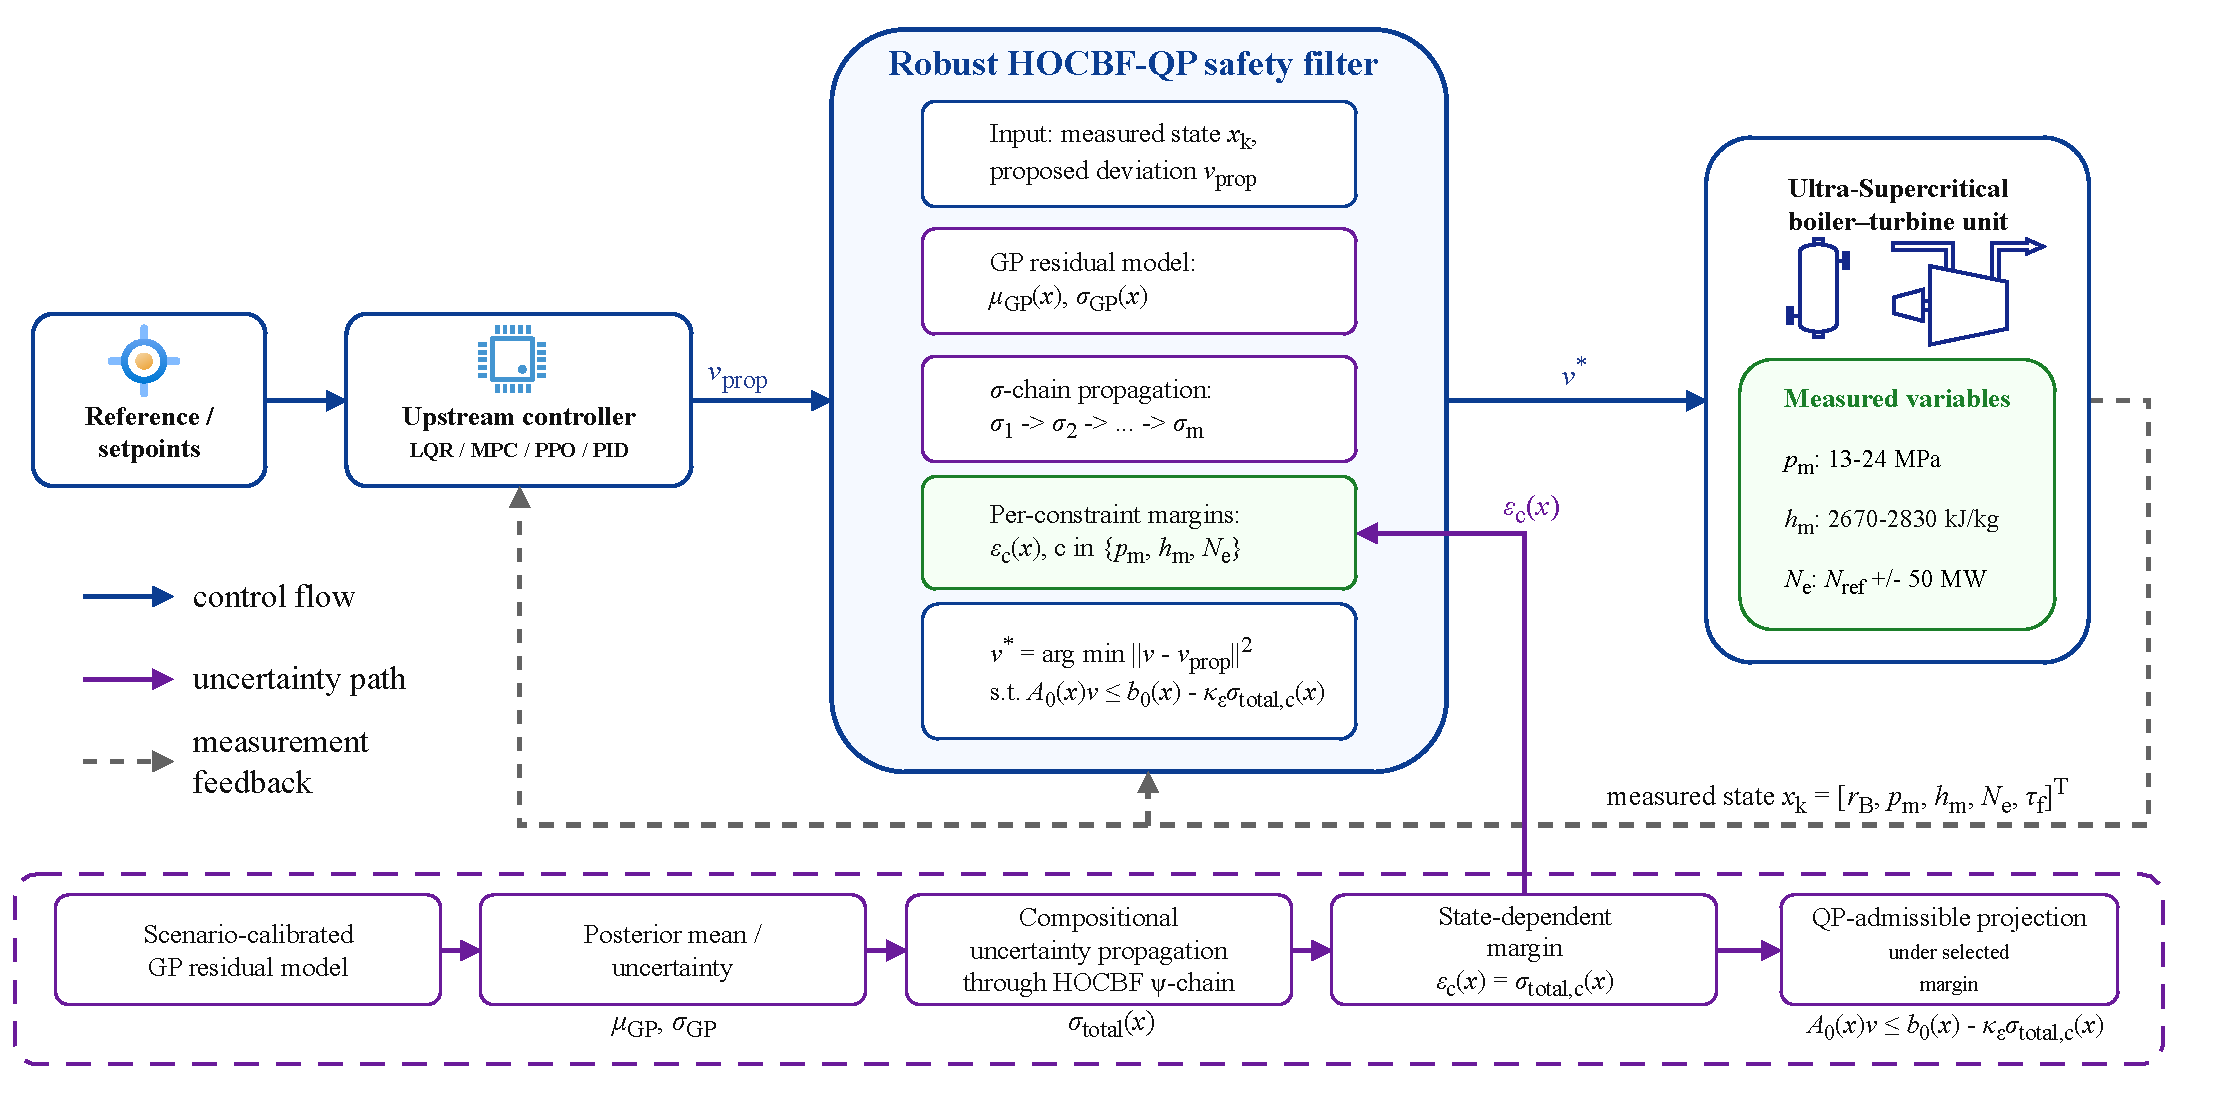
\includegraphics[width=1.00\textwidth]{figures/Figure_1.pdf}
    \caption{RoCBF-SF safety-filtering architecture. The upstream controller (LQR, MPC, PID, or learned policy) proposes a deviation command $v_{\mathrm{prop}}$. The filter evaluates that command against current plant measurements and the GP residual model, then projects it to the nearest QP-admissible deviation command $v^*$ under the selected margin through $A(x)v \leq b(x)-\epsilon_\kappa\sigmatotal(x)$. The physical actuator command is then reconstructed by Eq.~\eqref{eq:deviation_control}.}
    \label{fig:architecture}
\end{figure}

Figure~\ref{fig:architecture} provides the system map for the rest of the paper. Figure~\ref{fig:process_response} follows the signal path through plant response and QP intervention, and Fig.~\ref{fig:model_mismatch} checks the residual-model evidence for GP correction.

\subsection{GP Residual Correction and Compositional Margin}

Each modeled component of $\Deltaf_j$, $j\in J_{\mathrm{GP}}$, is represented by an independent GP with a Mat\'{e}rn-5/2 kernel. Kernel distances use the frozen training transform $\widetilde{x}_i=(x_i-\mu_{x_i}^{\mathrm{train}})/s_{x_i}^{\mathrm{train}}$; the standard-deviation floor is $10^{-6}$ of the corresponding engineering range. Residual targets are standardized separately for each output. The same frozen transforms are used for training, validation, and inference. Given $N$ training points, the posterior provides mean $\mu_{\mathrm{GP},j}(x)$ and variance $\sigma_{\mathrm{GP},j}^2(x)$. The formal analysis conditions on the simultaneous residual event
\begin{equation}
    |\Deltaf_j(x) - \mu_{\mathrm{GP},j}(x)| \leq \beta \sigma_{\mathrm{GP},j}(x),
    \quad j\in J_{\mathrm{GP}},\ x\in\calX_{\mathrm{op}},
\label{eq:gp_bound}
\end{equation}
with joint probability at least $1-\delta$. A standard RKHS sufficient multiplier includes both a residual RKHS-norm bound $B_\Delta$ and a sub-Gaussian noise scale $R$, for example $\beta_{\mathrm{RKHS}}=B_\Delta+R\sqrt{2(\gamma_N+1+\ln(q/\delta))}$ for $q=|J_{\mathrm{GP}}|$ modeled outputs~\cite{chowdhury2017kernelized}. The numerical studies and deployed configuration instead retain the fixed commissioning multiplier $\beta_{\mathrm{comm}}=\sqrt{2(\gamma_N+1+\ln(q/\delta))}$. This engineering scaling rule defines the reported posterior envelope but does not, by itself, establish Eq.~\eqref{eq:gp_bound}; Theorem~\ref{thm:1} applies only when that event is independently valid.

We define the mean-corrected drift $\fhat = f_0 + \muGP$ and posterior residual $\Delta \hat{f} = \Deltaf - \muGP$. The induced perturbation is propagated level by level through the HOCBF chain rather than attached only to the final constraint row.

The perturbation at level $i$ is $\delta_i = \psi_i - \hat{\psi}_i^0$, satisfying:
\begin{align}
    \delta_1 &= L_{\Delta\hat{f}}h \label{eq:d1}\\
    \delta_i &= L_{\Delta\hat{f}}\hat{\psi}_{i-1}^0 + (L_{\fhat}+k_i)\delta_{i-1} + L_{\Delta\hat{f}}\delta_{i-1}, \; i\geq 2 \label{eq:di}
\end{align}
This two-line recursion separates the nominal HOCBF recursion from mismatch residuals.

The compositional margin is constructed as:
\begin{subequations}
\label{eq:margin}
\begin{align}
    \sigma_1(x) &= \beta \sum_j |\partial h/\partial x_j| \sigmaGPj{j}(x), \label{eq:s1}\\
    \sigma_i(x) &= \beta \sum_j |\partial \hat{\psi}_{i-1}^0/\partial x_j| \sigmaGPj{j}(x)
    +(\|L_{\fhat}\|_{\mathrm{op}}+k_i)\sigma_{i-1}(x)
    +\sigma_{\mathrm{cross}}^{(i)}(x),\quad i\geq 2, \label{eq:si}\\
    \sigmatotal(x) &= \sigma_m(x)+\sum_{j=1}^{m-1}c_j\sigma_j(x)+\sigma_{\mathrm{ctrl}}(x). \label{eq:st}
\end{align}
\end{subequations}
The three margin relations above define the quantity scaled by $\epsilon_\kappa$ in the online QP. For the formal result, $\|L_{\fhat}\|_{\mathrm{op}}$ is a uniform operating-set bound and $\sigma_{\mathrm{cross}}^{(i)}$ must bound $|L_{\Delta\hat f}\delta_{i-1}|$; Lemma~S1 gives a sufficient derivative-bound construction. The numerical implementation uses the nominal stabilized drift in the uncertainty recursion and the commissioning proxy $\sigma_{\mathrm{cross,comm}}^{(i)}(x)=\beta_{\mathrm{comm}}\|\nabla\hat{\psi}_{i-1}^0(x)\|_2\|\sigmaGP(x)\|_2$. In the linear stabilized benchmark, the nominal drift-Jacobian norm is global. For a nonlinear deployment, an equilibrium Jacobian is only a local engineering estimate. Neither the proxy cross term nor a local Jacobian estimate is automatically a certificate bound; Assumption~\ref{ass:residual_bound} states the additional dominance condition required by Theorem~\ref{thm:1}. The control-coupling term is
\begin{equation}
    \sigma_{\mathrm{ctrl}}(x)=\beta\sum_j\left|\frac{\partial(L_gL_{\fhat}^{m-1}h)}{\partial x_j}\right|\sigmaGPj{j}(x)u_{\max},
    \label{eq:sigma_ctrl_main}
\end{equation}
where $u_{\max}=\sup_{u\in\calU}\|u\|$. The chain weights are $c_j=\prod_{\ell=j+1}^{m-1}(\|L_{\fhat}\|_{\mathrm{op}}+k_\ell)$, with the empty product equal to one; thus $c_1=1$ for the pressure barriers with $m=2$. The resulting HOCBF constraint is $A_0(x)v \leq b_0(x)-\epsilonKappa\sigmatotal(x)$.

\subsection{Commissioning Factor and Implementation Boundary}

\begin{assumption}[Operating set and relative degree]
\label{ass:operating_set}
The state remains in a compact operating set $\calX_{\mathrm{op}}\subset\calX$, the barriers in Eq.~\eqref{eq:barriers} are continuously differentiable to the required HOCBF order, and their relative degrees are known on $\calX_{\mathrm{op}}$.
\end{assumption}

\begin{assumption}[Drift-residual GP event]
\label{ass:gp_event}
The input matrix is exact ($\Delta g=0$). For the $q=3$ modeled residual outputs $J_{\mathrm{GP}}=\{p_m,h_m,N_e\}$, Eq.~\eqref{eq:gp_bound} holds simultaneously over $\calX_{\mathrm{op}}$ with probability at least $1-\delta$. This event may be established from valid RKHS and noise bounds or another justified uniform-error result; the commissioning multiplier $\beta_{\mathrm{comm}}$ alone is not such a proof. Residuals in the unmodeled $r_B$ and $\tau_f$ rows are zero in the drift-only benchmark or are otherwise covered by Assumption~\ref{ass:residual_bound}.
\end{assumption}

\begin{assumption}[Compositional residual bound]
\label{ass:residual_bound}
The derivative constants used in Lemma~S1 are finite on $\calX_{\mathrm{op}}$, the operator-norm and cross-term quantities are valid upper bounds rather than local proxies, and the margin definitions in Section~3.3, together with Eq.~\eqref{eq:sigma_ctrl_main}, satisfy $|\Delta_{\psi}(x,v)|\leq\sigmatotal(x)$ for every active HOCBF row and every admissible $v\in\mathcal{V}$.
\end{assumption}

\begin{assumption}[Robust-QP feasibility]
\label{ass:qp_feasible}
For every $x\in\calX_{\mathrm{op}}$ considered by the certificate, there exists at least one $v\in\mathcal{V}$ satisfying $A(x)v\leq b(x)-\sigmatotal(x)$.
\end{assumption}

\begin{theorem}[Conditional probabilistic forward invariance]
\label{thm:1}
Let $\Delta_{\psi}(x,v)=\psi_m^{\mathrm{true}}(x,v)-\hat{\psi}_m^0(x,v)$ denote the induced top-level HOCBF residual after substituting the deviation-input model. Under Assumptions~\ref{ass:operating_set}--\ref{ass:qp_feasible}, the QP in Eq.~\eqref{eq:online_qp} with $\epsilonKappa=1$ renders $\calC$ forward invariant with probability at least $1-\delta$.
\end{theorem}

\noindent\textit{Proof.}
The complete proof is given in the Supplemental Material. It conditions on the simultaneous residual event, applies the derivative-bound construction in Lemma~S1, invokes Assumption~\ref{ass:residual_bound} to obtain $|\Delta_\psi(x,v)|\leq\sigmatotal(x)$, and then applies the HOCBF forward-invariance result to the tightened QP. The certificate is attached to $\epsilon_\kappa=1$, independently valid residual and derivative bounds, and robust-QP feasibility.

Theorem~\ref{thm:1} is a conditional worst-case statement. The margin itself does not imply feasibility; feasibility depends on safe-set geometry, actuator limits, and $\calU$. The online factor $\epsilon_\kappa$ therefore has a dual interpretation: at $\epsilon_\kappa=1$ it applies the complete implemented margin and recovers the formal bound only when Assumptions~\ref{ass:gp_event}--\ref{ass:qp_feasible} are established; smaller values are commissioning settings selected from replay and operating-envelope diagnostics.

The robustness scaling factor $\epsilon_\kappa$ controls the safety-margin/control-authority trade-off:

\begin{itemize}
    \item $\epsilon_\kappa = 0$: The QP enforces $A_0(x)v \leq b_0(x)$, i.e., the nominal HOCBF constraint with GP mean correction only. No robustness margin is applied beyond the mean correction itself.
    \item $\epsilon_\kappa = 1$: The QP enforces the full implemented compositional margin $\sigmatotal(x)$. It recovers the worst-case certificate only when the residual event, derivative bounds, $\Delta g=0$, and full-row QP feasibility required by Theorem~\ref{thm:1} all hold.
    \item $0 < \epsilon_\kappa < 1$: The QP enforces a fraction of the compositional margin, trading theoretical coverage for reduced QP conservatism.
\end{itemize}

The conditional probabilistic certificate is available only at $\epsilon_\kappa=1$ when every assumption of Theorem~\ref{thm:1} is established; setting $\epsilon_\kappa=1$ alone is insufficient. Values $0 \leq \epsilon_\kappa < 1$ are calibrated operating points evaluated by finite-sample violation, QP intervention, infeasibility, and deployment-envelope diagnostics. Section~\ref{sec:exp} evaluates the full implemented-margin endpoint in the actuator-limited benchmark and how the preferred value changes with mismatch structure.

The GP posterior includes a regularization floor $\sigma_{\mathrm{floor}}=10^{-4}$. Under constant perturbations, $\sigmaGP$ and $\sigmatotal(x)$ are nearly uniform, so the margin is floor-driven. Under S3 state-dependent coupling, $\sigmaGP$ becomes heterogeneous and $\sigmatotal(x)$ is data-driven. This distinction explains why additive perturbations can use $\epsilon_\kappa=0$ in the tested regime: GP mean correction supplies the effective adjustment, while the floor-driven margin mainly adds QP conservatism.

Theorem~\ref{thm:1} is continuous-time, whereas the implementation uses $T_s = 1$\,s zero-order hold. One second is the deployed coordinated-control task period and allows the filter to evaluate each upstream command update; it is not intended to imply that the dominant boiler thermal dynamics have a 1\,s time constant. The deployed task deadline is 1000\,ms and the configured QP timeout is 200\,ms; the observed controller-task and QP times are reported separately in Section~\ref{sec:historian}. The 5\,s spacing in the controller exports is a logging interval rather than the internal execution period. A failed original QP permits at most one reduced-QP attempt after removal of the whitelisted \texttt{pressure\_low} row, and only when $\|G_iS_u\|_2<0.01$, the unscaled row right-hand side is below $-10^{-6}$, the directly measured pressure margin is at least 2.0\,MPa, measurement quality is good, and no protection or interlock is active. Actuator box/rate rows are never removed. A failed retry, hard fault, or timeout returns the live coordinated-control command and latches bypass according to the deployment state machine. The reduced-QP recovery does not satisfy Assumption~\ref{ass:qp_feasible} for the original six-row problem, so Theorem~\ref{thm:1} does not apply during those recovered cycles. Inter-sample forward invariance is not established by the reported controller-instant tests and remains outside the formal certificate.

For field commissioning, approximately 14 days of 1\,Hz data are divided into days 1--10 for the training candidate pool, day 11 as a 24\,h isolation gap, and days 12--14 for validation. Five fixed load strata cover 180--660\,MW; each contributes 100 training and 40 validation transitions. Within each stratum, candidates are thinned to at least 60\,s spacing and selected by deterministic farthest-point coverage in standardized $(p_m,h_m,N_e)$ coordinates, without quota borrowing. The deployed dictionary is frozen at 500 points. Plant-specific training-block replay fixes $\epsilon_\kappa=0.1$, after which the 200 time-isolated validation points are evaluated once without retuning. The public controller exports confirm the implemented value and online execution; the record-level plant replay remains a restricted enterprise asset and is not reconstructed from those exports.

Coverage monitoring combines the input z-score and 0.5th--99.5th training quantiles, the validation-set 99th percentile of posterior standard deviation, and the standardized one-step innovation. Moderate OOD enters full-row nominal-HOCBF operation for at most ten 1\,s cycles; GP operation resumes only after ten consecutive healthy cycles. A persistent coverage failure enters latched live-DCS bypass. Innovation above 5, invalid measurements or communication, non-finite/model-load faults, nominal-QP or actuator-constraint infeasibility, violation of a direct physical bound, pressure-low physical margin below 2.0\,MPa, or QP/task timeout bypasses the degraded stage immediately. This nominal-HOCBF interval is a bounded transition mode without a GP coverage claim, not a certified substitute for the GP-RHOCBF mode.
